\documentclass[12pt]{article}
\usepackage{times} 			% use Times New Roman font

\usepackage[margin=1in]{geometry}   % sets 1 inch margins on all sides
\usepackage[hidelinks]{hyperref}               % for URL formatting
\usepackage[pdftex]{graphicx}       % So includegraphics will work
\setlength{\parskip}{1em}           % skip 1em between paragraphs
\usepackage{indentfirst}            % indent the first line of each paragraph
\usepackage{datetime}
\usepackage[small, bf]{caption}
\usepackage{listings}               % for code listings
\usepackage{xcolor}                 % for styling code
\usepackage{multirow}
\usepackage{subcaption}     % for subfigures

%\setlength\intextsep{1.69cm} 

%New colors defined below
\definecolor{backcolour}{RGB}{246, 246, 246}   % 0xF6, 0xF6, 0xF6
\definecolor{codegreen}{RGB}{16, 124, 2}       % 0x10, 0x7C, 0x02
\definecolor{codepurple}{RGB}{170, 0, 217}     % 0xAA, 0x00, 0xD9
\definecolor{codered}{RGB}{154, 0, 18}         % 0x9A, 0x00, 0x12

%Code listing style named "gcolabstyle" - matches Google Colab
\lstdefinestyle{gcolabstyle}{
  basicstyle=\ttfamily\small,
  backgroundcolor=\color{backcolour},   
  commentstyle=\itshape\color{codegreen},
  keywordstyle=\color{codepurple},
  stringstyle=\color{codered},
  numberstyle=\ttfamily\footnotesize\color{darkgray}, 
  breakatwhitespace=false,         
  breaklines=true,                 
  captionpos=b,                    
  keepspaces=true,                 
  numbers=left,                    
  numbersep=5pt,                  
  showspaces=false,                
  showstringspaces=false,
  showtabs=false,                  
  tabsize=2
}

\lstset{style=gcolabstyle}      %set gcolabstyle code listing

% to make long URIs break nicely
\makeatletter
\g@addto@macro{\UrlBreaks}{\UrlOrds}
\makeatother

% for fancy page headings
\usepackage{fancyhdr}
\setlength{\headheight}{13.6pt} % to remove fancyhdr warning
\pagestyle{fancy}
\fancyhf{}
\rhead{\small \thepage}
\chead{\small CS 532, Spring 2024} 
\lhead{\small EC 0.6 - Reports , Thennakoon}  % EDIT THIS, REPLACE # with HW number

%-------------------------------------------------------------------------
\begin{document}

% EDIT THE ITEMS HERE
\begin{centering}
{\large\textbf{EC 0.6 - Reports}}\\ 
Kumushini Thennakoon\\
2024-01-21\\
\end{centering}

%-------------------------------------------------------------------------

% The * after \section just says to not number the sections
\section*{Q1}

\emph{You may copy the question into your report, but make sure that you make it clear where the question ends and your answer begins.}

\subsection*{Answer}

\emph{All figures must have a caption and must be referenced in the text. Example below.}

Figure \ref{fig:web-growth} shows the growth in the number of websites between 1993 and 1996.

\begin{figure}[h!]
    \centering
    % trim and clip are used to crop the image, trim=left bottom right top
    % width sets max width, height will be scaled appropriately
    \fbox{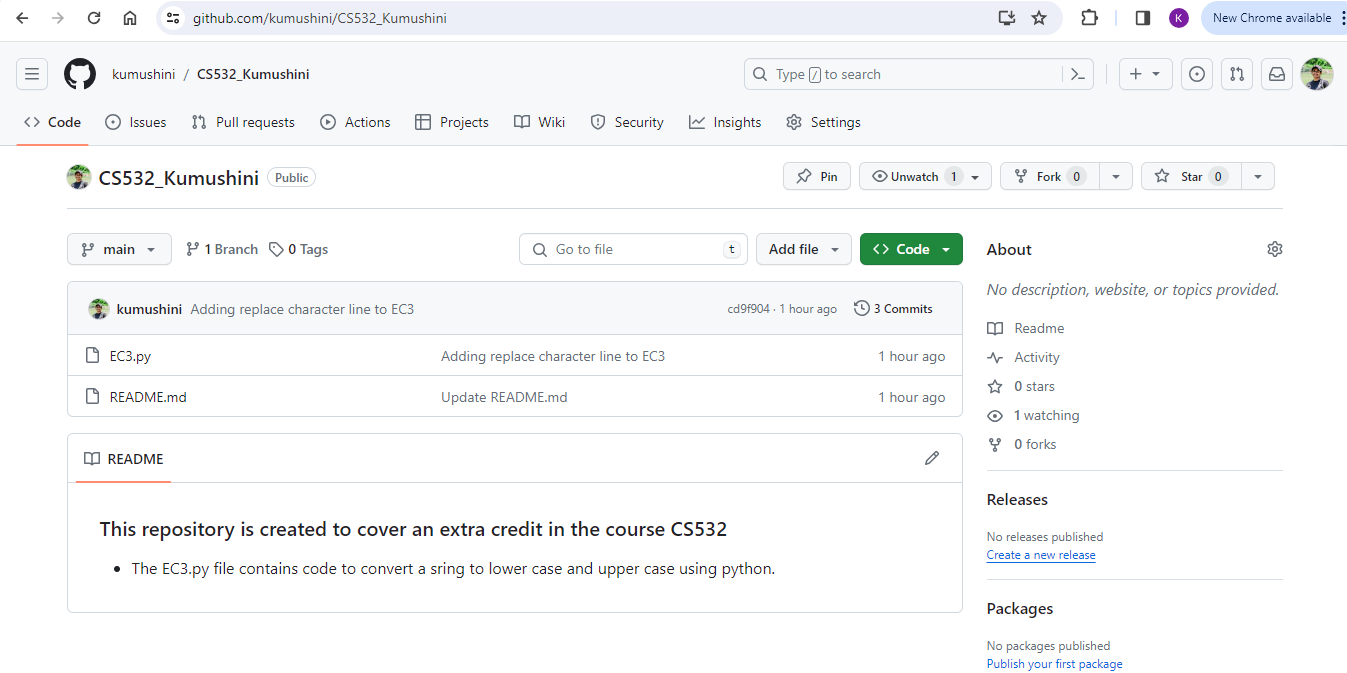
\includegraphics[trim=0 20 10 50, clip, width=\textwidth] {GitHub_repo_kumushini.png}}
    \caption{Image of the Kumushini's GitHub repository created for CS 532 course}
    \label{fig:web-growth}
\end{figure}

\emph{If you want to include code in your report, you can insert a screenshot (if it's legible), or you can copy/paste the code into a listings environment. There are examples below and more information is available at \url{https://www.overleaf.com/learn/latex/code_listing}.}

Listing \ref{lst:copy} is an example of directly copying code into the LaTeX document and having the listings package perform syntax highlighting. Listing \ref{lst:import} is an example of importing the code from a file rather than copying it in.

%Python code highlighting
\begin{lstlisting}[language=Python, caption=Python example copied into the LaTeX, label=lst:copy]
#!/usr/bin/python3
#EC3.py

a = "Hello, World!"
print(a.lower())
\end{lstlisting}

%Importing code from file
\lstinputlisting[language=Python, caption=Python sample code loaded from file, label=lst:import]{EC3.py}

Table \ref{tbl:simple} shows a simple example table.  Table \ref{tbl:confusion} shows an example confusion matrix (you'll see this term later) from \url{https://en.wikipedia.org/wiki/Confusion_matrix}. This employs rows that span multiple columns (multicol) and columns that span multiple rows (multirow). 

\begin{table}[h]
\centering
\caption{Simple Table}
\label{tbl:simple}
\begin{tabular}{|l|l|l|}
\hline
\textbf{Week} & \textbf{Date} & \textbf{Topic} \\ \hline \hline
1 & Jan 6 & Introduction to Web Science and Web Architecture \\ \hline
2 & Jan 13 & Introduction to Python\\ \hline
3 & Jan 20 & Measuring the Web \\ \hline
4 & Jan 27 & Searching the Web \\ \hline
\end{tabular}
\end{table}

\begin{table}[h]
\centering
\caption{Example Confusion Matrix from Wikipedia}
\label{tbl:confusion}
\begin{tabular}{l|l|c|c|}
\multicolumn{2}{c}{}&\multicolumn{2}{c}{Actual}\\
\cline{3-4}
\multicolumn{2}{c|}{}&Cat&Dog\\
\cline{2-4}
\multirow{2}{*}{Predicted}& Cat & 5 (TP) & 3 (FP)\\
\cline{2-4}
& Dog & 2 (FN) & 3 (TN) \\
\cline{2-4}
\end{tabular}
\end{table}

\emph{You must provide some discussion of every answer. Discuss how you arrived at the answer and the tools you used. Discuss the implications of your answer.}

\section*{Q2}

\subsection*{Answer}

Figure \ref{fig:subfigure-ex} shows an example of grouping related figures into a subfigure.  This includes Figure \ref{fig:cnn-2015aug02} and Figure \ref{fig:cnn-2015oct01}.
\begin{figure}[ht]
\centering
\begin{subfigure}{0.45\textwidth}
  \centering
  \includegraphics[width=0.9\linewidth]{cnn-20150802-IA.png}
  \caption{Archived CNN.com from Aug 2, 2015, \url{https://web.archive.org/web/20150802000019/http://www.cnn.com/}.}
\label{fig:cnn-2015aug02}
\end{subfigure}
\hspace{20pt}
\begin{subfigure}{0.45\textwidth}
  \centering
  \includegraphics[width=0.9\linewidth]{cnn-20151001-IA.png}
  \caption{Archived CNN.com from Oct 1, 2015, \url{https://web.archive.org/web/20151001000018/http://www.cnn.com/}.}
\label{fig:cnn-2015oct01}
\end{subfigure}%
\caption{Content from Jul 10, 2015 appearing in replayed pages with Memento-Datetimes of Aug 2, 2015 and Oct 1, 2015.}
\label{fig:subfigure-ex}
\end{figure}

\section*{Q3}

\subsection*{Answer}

\section*{References}

\emph{Every report must list the references that you consulted while completing the assignment. If you consulted a webpage, you must include the URL.}

\begin{itemize}
    \item {Wikipedia, What is web science?, \url{https://en.wikipedia.org/wiki/Web_science}}
    \item{Google scholar,  Evolution of the world wide web: From WEB 1.0 TO WEB 4.0, \url{https://d1wqtxts1xzle7.cloudfront.net/57492902/ijwest_top_10-libre.pdf?1538542692=&response-content-disposition=inline%3B+filename%3DTOP_10_WEB_and_SEMANTIC_TECHNOLOGY_PAPER.pdf&Expires=1705891097&Signature=a7LeWE98gvVAbi10wMrnXKQ9Fnsfax1xZe9RSsBbc0LOTU~cUTVSyz2BtCEaJDR0hHrjjd7kSYUTxNBsRqOM6zvx3ZRKdeZkDe8gkcwdjpsdXvbw8EdatZhr16~FyOHqzSN~lMAh4v0QYsovhAK2MYDVe0pnPe51fOCBO6PsxsyCdzC5SMqh0JvGjHbVuCOSaILMbNm8yBsPaf-LFD1w8njREETAuCVPlb1HP3ZOf55HxpNKL1DonZ2mFpAXDZ4~KMva9P7mJkV6PAQa45GV8KH702mqMad9HqsCrZb00DX9UkzX459ETFeoF-5-DN2FNKx5ZST38KdP9rFyi1hLaA__&Key-Pair-Id=APKAJLOHF5GGSLRBV4ZA}}
     \item {You tube, Web security, \url{https://www.youtube.com/watch?v=5JJrJGZ_LjM&list=PL1y1iaEtjSYiiSGVlL1cHsXN_kvJOOhu-}}
\end{itemize}

\end{document}

